\documentclass{article}
\usepackage[margin=1in]{geometry}
\usepackage{graphicx}
\usepackage{float}
\begin{document}
\section*{S7.3(A)}
\begin{figure}[H]
\centering
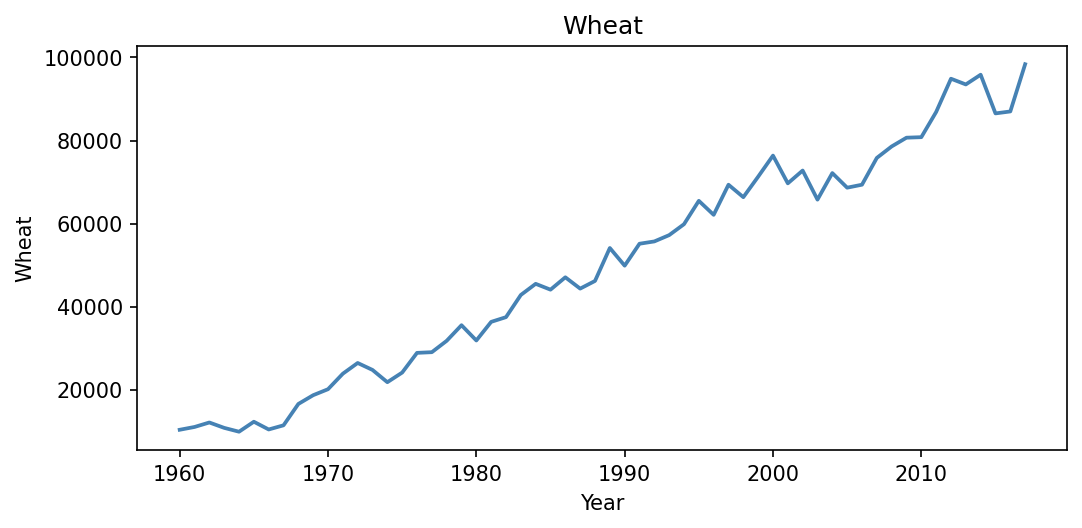
\includegraphics[width=0.95\linewidth]{S7.3A_wheat_ts.png}
\caption{Time-series plot of wheat}
\end{figure}
\begin{figure}[H]
\centering
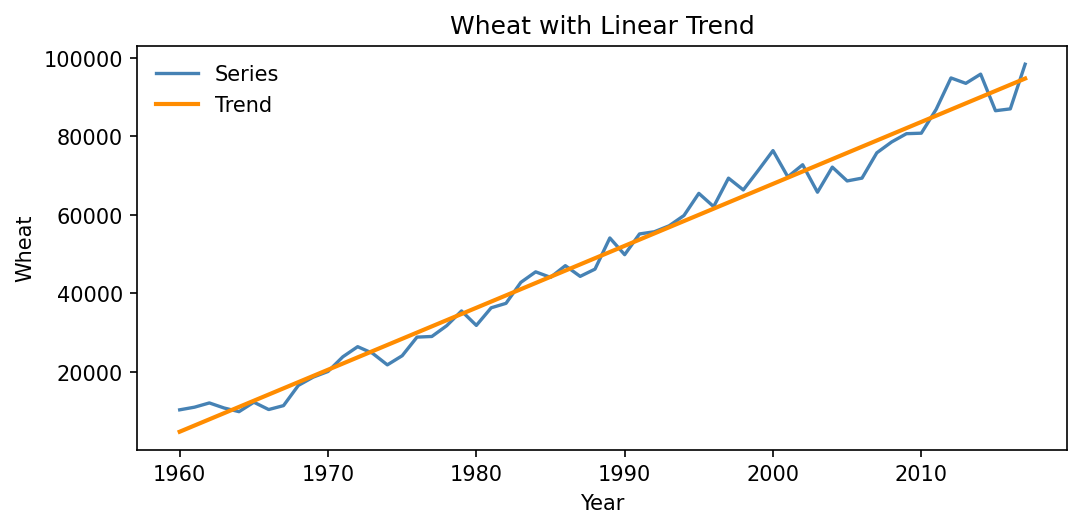
\includegraphics[width=0.95\linewidth]{S7.3A_wheat_trend.png}
\caption{Wheat with a quadratic deterministic trend}
\end{figure}
The series shows a strong upward deterministic trend. A linear trend in time fits nearly as well as a quadratic one; AIC/BIC slightly favor the linear specification. A log-linear trend is also plausible if growth is proportional. Economically, the trend is consistent with technological improvements (Green Revolution), expanded irrigation, fertilizer use, improved seed varieties, and policy support that raised yields and production over time.
(exponential growth) or a quadratic trend in time; the quadratic captures visible curvature in levels. 
Economically, the trend is consistent with technological improvements (Green Revolution), expanded irrigation, 
fertilizer use, improved seed varieties, and policy support that raised yields and production over time.
\begin{table}[H]
\centering
\begin{tabular}{lrrrr}
\hline
Method & RMSE & AIC & BIC & $n$ \\
\hline
linear & 3756.459 & 1123.420 & 1127.541 & 58 \\
quadratic & 3744.537 & 1125.051 & 1131.232 & 58 \\
cubic & 3744.701 & 1125.056 & 1131.237 & 58 \\
log-linear & 10548.084 & -17.531 & -13.411 & 58 \\
log-quadratic & 4225.527 & -95.285 & -89.103 & 58 \\
hp & 3516.936 &  &  & 58 \\
moving\_average & 2345.683 &  &  & 58 \\
lowess & 3217.104 &  &  & 58 \\
\hline
\end{tabular}
\caption{Trend fit summary for wheat}
\end{table}
\end{document}
